\documentclass[11pt,a4paper]{article}
\usepackage[T1]{fontenc}
\usepackage[margin=2.3cm]{geometry}
\usepackage{amsmath,amssymb}
\usepackage{graphicx}
\usepackage[dvipsnames]{xcolor}
\usepackage{enumitem}
\usepackage[colorlinks=true,linkcolor=blue,urlcolor=blue]{hyperref}
\setlength{\parskip}{0.6em}
\setlength{\parindent}{0pt}
\begin{document}

\begin{center}{\LARGE\bfseries opencircuitlab}\\[0.4em]{\large Build series and parallel circuits and solve them with Kirchhoff's laws.}\\[0.2em]\small PAN IIT OSS explainer \textbullet{} secondary school to diploma / undergraduate (levels 3-5)\end{center}

\section*{Why this exists}
Every circuit, from a torch to a sensor board, obeys two simple conservation laws. This explainer shows how they turn into one matrix equation, so that any resistor network can be solved by a few lines of Python.

\section*{The end goal}
Build series and parallel circuits and solve them with Kirchhoff's laws. The end goal is to build series and parallel circuits and solve them with Kirchhoff's laws: by hand for small circuits, and with a nodal-analysis solver for any network, validated against hand results and against energy conservation. The same method sits inside circuit simulators used throughout electronics.

\section*{How the three sessions build up}
\begin{enumerate}[nosep]
\item \textbf{Session 1: A battery, a switch and bulbs: series and parallel} (Level 1, conceptual interactive model, 60 min).
\item \textbf{Session 2: Kirchhoff's laws, dividers and the loading effect} (Level 2, mathematical engineering model, 80 min).
\item \textbf{Session 3: Nodal analysis by matrix, Thevenin and the sensor bridge} (Level 3, simulation and validation, 90 min).
\end{enumerate}

\section{Session 1: A battery, a switch and bulbs: series and parallel}

\subsection*{A. Real-world problem}
Old festival lights were wired in one long chain: when one bulb burned out, the whole string went dark, and when you added more bulbs, all of them got dimmer. A torch with two bulbs on the same battery behaves differently. Why does the same battery make bulbs glow dim in one wiring and bright in another, and what does the battery pay for the brightness? (Low-voltage educational circuits only: never experiment with mains electricity.)

\subsection*{B. Concept and theory}
A battery pushes charge round a closed loop. In a series chain there is only one path, so the same current passes through every bulb, one after another; the resistances add up and the battery voltage is shared between the bulbs. In a parallel bank every bulb is connected straight across the battery, so each gets the full voltage and carries its own current; the battery has to supply all those currents together. Power in a bulb is P = V I = I\textasciicircum{}2 R = V\textasciicircum{}2 / R, and we take brightness to be proportional to it. A switch is just a gap: open means no loop and no current.

\begin{itemize}[nosep]
\item V: battery voltage (V)
\item R: resistance of one bulb (model value 10) (ohm)
\item N: number of identical bulbs (no unit)
\item I: current drawn from the battery (A)
\item P: power in one bulb (heat and light) (W)
\end{itemize}

\begin{equation*}
I=\frac{V}{R}\qquad P=VI=I^2R=\frac{V^2}{R}
\end{equation*}

\begin{equation*}
\text{series: } R_{\mathrm{tot}}=NR,\quad I=\frac{V}{NR},\quad V_{\mathrm{bulb}}=\frac{V}{N},\quad P_{\mathrm{bulb}}=\frac{V^2}{N^2R}
\end{equation*}

\begin{equation*}
\text{parallel: } R_{\mathrm{tot}}=\frac{R}{N},\quad I=\frac{NV}{R},\quad V_{\mathrm{bulb}}=V,\quad P_{\mathrm{bulb}}=\frac{V^2}{R}
\end{equation*}

\begin{center}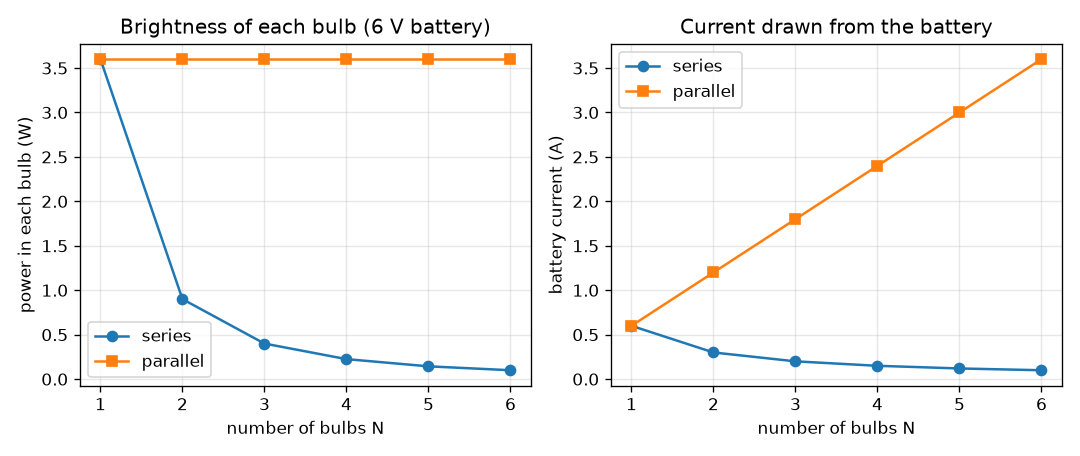
\includegraphics[width=0.85\linewidth]{figures/s01_bulbs_compare.png}\\\small Each bulb's power and the battery current for 1 to 6 bulbs on 6 V, in series and in parallel.\end{center}

\subsection*{E. Worked example}
A 6 V battery feeds three bulbs of 10 ohm each. Find the current, the voltage across each bulb and its power for (a) the series wiring and (b) the parallel wiring.
\begin{enumerate}[nosep]
\item Series: R\_total = 3 * 10 = 30 ohm, so I = 6 / 30 = 0.2 A, the same in every bulb.
\item Voltage across each bulb = I R = 0.2 * 10 = 2 V (three of them add to 6 V, as they must).
\item Power in each bulb = V I = 2 * 0.2 = 0.4 W; total 1.2 W, which equals battery voltage times current, 6 * 0.2.
\item Parallel: each bulb sees 6 V, so its current is 6 / 10 = 0.6 A and its power is 6 * 0.6 = 3.6 W.
\item The battery supplies 3 * 0.6 = 1.8 A and 10.8 W in total. Parallel gives each bulb 9 times the power of series, since the voltage is 3 times larger and power goes with the square.
\end{enumerate}
\textbf{Answer.} Series: 0.2 A, 2 V and 0.4 W per bulb. Parallel: 1.8 A from the battery, 6 V and 3.6 W per bulb.

\subsection*{F. Questions}
\begin{enumerate}[nosep]
\item \textbf{Conceptual.} In a series string of festival bulbs, one bulb fails by breaking its filament. Why do all the other bulbs go out, and why would they stay lit in a parallel string?
\item \textbf{Numerical.} A 9 V battery feeds three 10 ohm bulbs. Find the current and the power in each bulb for the series wiring and for the parallel wiring.
\item \textbf{Graph and simulation interpretation.} On the brightness graph at 6 V, how many times dimmer is each bulb for 4 bulbs in series than for 4 bulbs in parallel? Read the two values from the curves.
\item \textbf{Design and optimisation challenge.} Design: a small 6 V battery can supply at most 1 A. You must light three 10 ohm bulbs and want each to get at least 0.3 W. Compare three wirings: all series, all parallel, and one bulb in series with a parallel pair. Which are allowed, and which would you choose?
\end{enumerate}

\section{Session 2: Kirchhoff's laws, dividers and the loading effect}

\subsection*{A. Real-world problem}
A microcontroller board runs on 3.3 V, but your battery pack gives 5 V. Two resistors can drop the voltage, and they do it perfectly until you connect the sensor: then the output sags to 2.7 V and the board misbehaves. And what if a second battery is connected to the same circuit, and the current in it flows the 'wrong' way? You need two laws that always hold, and a design method. (Low-voltage educational circuits only; this is a simplified model, not a design for real equipment.)

\subsection*{B. Concept and theory}
Kirchhoff's current law: at any node (a point where wires meet) the currents flowing in equal the currents flowing out, because charge does not pile up. Kirchhoff's voltage law: going once round any closed loop, the voltage rises and drops add up to zero, because energy is conserved. A voltage divider is two resistors in series across V\_in: the same current I = V\_in / (R1 + R2) flows through both, so V\_out across R2 is V\_in R2 / (R1 + R2). A current divider splits a total current between two parallel branches: the smaller resistor takes the larger share. A load R\_L across R2 puts R\_L in parallel with it, which lowers the lower resistance and so lowers V\_out: this is the loading effect. For a circuit with two loops, write KVL for each loop with the loop currents as unknowns and solve the two equations together; a negative answer means the current really flows the other way. For a design, work backwards: the loaded lower resistance must equal R1 V\_target / (V\_in - V\_target), and R2 is found from R2 \textbar{}\textbar{} R\_L.

\begin{itemize}[nosep]
\item V\_in: input voltage (5) (V)
\item V\_out: voltage across the lower resistor and the load (V)
\item R1, R2: upper and lower divider resistors (ohm)
\item R\_L: load resistance connected across R2 (ohm)
\item I1, I2: currents delivered by battery 1 and battery 2 (A)
\item V\_A: voltage of the node where both batteries and R3 meet (V)
\end{itemize}

\begin{equation*}
\sum I_{\mathrm{in}}=\sum I_{\mathrm{out}}\ \text{(KCL)}\qquad \sum V_{\mathrm{loop}}=0\ \text{(KVL)}
\end{equation*}

\begin{equation*}
V_{\mathrm{out}}=V_{\mathrm{in}}\frac{R_2}{R_1+R_2}\qquad I_1=I_t\frac{R_2}{R_1+R_2}
\end{equation*}

\begin{equation*}
V_{\mathrm{out}}=V_{\mathrm{in}}\frac{R_2\parallel R_L}{R_1+R_2\parallel R_L},\qquad R_2\parallel R_L=\frac{R_2R_L}{R_2+R_L}
\end{equation*}

\begin{equation*}
\begin{pmatrix}R_1+R_3 & R_3\\ R_3 & R_2+R_3\end{pmatrix}\begin{pmatrix}I_1\\ I_2\end{pmatrix}=\begin{pmatrix}V_1\\ V_2\end{pmatrix}
\end{equation*}

\begin{equation*}
\frac{1}{R_2}=\frac{1}{R_{\mathrm{low}}}-\frac{1}{R_L},\qquad R_{\mathrm{low}}=\frac{R_1V_{\mathrm{target}}}{V_{\mathrm{in}}-V_{\mathrm{target}}}
\end{equation*}

\begin{center}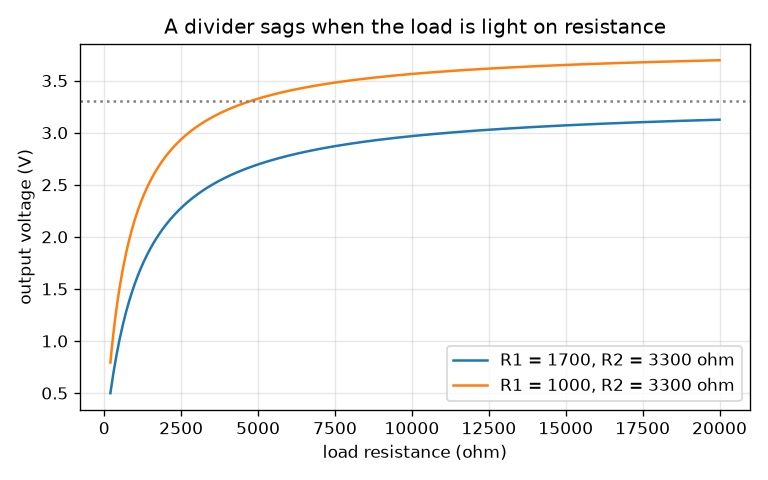
\includegraphics[width=0.85\linewidth]{figures/s02_divider_loading.png}\\\small Output of a 5 V divider against the load resistance: a divider is only 'stiff' for light loads.\end{center}

\subsection*{E. Worked example}
Battery 1 (V1 = 10 V) with R1 = 100 ohm and battery 2 (V2 = 4 V) with R2 = 200 ohm both feed node A; R3 = 300 ohm connects A to ground. Find I1, I2, the voltage V\_A, and check with KCL, KVL and power.
\begin{enumerate}[nosep]
\item Let I1 and I2 flow from the batteries towards A, so R3 carries I1 + I2. KVL on loop 1: 10 = 100 I1 + 300 (I1 + I2), that is 400 I1 + 300 I2 = 10.
\item KVL on loop 2: 4 = 200 I2 + 300 (I1 + I2), that is 300 I1 + 500 I2 = 4.
\item Determinant = 400 * 500 - 300 * 300 = 110000. I1 = (10 * 500 - 300 * 4) / 110000 = 3800 / 110000 = 0.034545 A. I2 = (400 * 4 - 300 * 10) / 110000 = -1400 / 110000 = -0.012727 A.
\item R3 carries I1 + I2 = 0.021818 A, so V\_A = 300 * 0.021818 = 6.545 V. I2 is negative: battery 2 (4 V) is being charged by battery 1 because V\_A is above 4 V.
\item Checks. KVL loop 2: 4 - 200 * (-0.012727) - 6.545 = 4 + 2.545 - 6.545 = 0. Power supplied: 10 * 0.034545 + 4 * (-0.012727) = 0.29455 W; dissipated: 0.11934 + 0.03240 + 0.14281 = 0.29455 W.
\end{enumerate}
\textbf{Answer.} I1 = 34.55 mA, I2 = -12.73 mA (battery 2 is charged), V\_A = 6.545 V; the power balance is 294.5 mW supplied and 294.5 mW dissipated.

\subsection*{F. Questions}
\begin{enumerate}[nosep]
\item \textbf{Conceptual.} Why does connecting a load always lower the output of a voltage divider, and when can you safely ignore the load?
\item \textbf{Numerical.} A 9 V source feeds R1 = 2 kohm in series with R2 = 1 kohm. Find the unloaded output, then the output with a 1 kohm load across R2. Check both with KVL.
\item \textbf{Graph and simulation interpretation.} In the loading graph for R1 = 1700 ohm and R2 = 3300 ohm, at roughly what load resistance does the output fall to 3.0 V (about 9 percent below the target)? Which direction does the curve move if R2 is made smaller?
\item \textbf{Design and optimisation challenge.} Design: the output must be exactly 3.3 V from 5 V with a 4.7 kohm load. Compare R1 = 220 ohm, 470 ohm and 1000 ohm. For each, find R2, the source current and the error if the load is later unplugged. Which do you choose and why?
\end{enumerate}

\section{Session 3: Nodal analysis by matrix, Thevenin and the sensor bridge}

\subsection*{A. Real-world problem}
A temperature sensor on a board is a resistor whose value changes by a fraction of a percent per degree. A Wheatstone bridge turns that tiny change into a measurable voltage, but every other resistor in the bridge is only guaranteed to 5 percent. Hand solving is already painful for three loops; real boards have hundreds of nodes. How do we let the computer solve any network, trust the answer, and predict how badly component tolerance spoils a measurement? (Low-voltage educational circuits only; this is a simplified model, not a design tool for real equipment.)

\subsection*{B. Concept and theory}
Number the nodes and choose one as the 0 V reference. A resistor R between nodes a and b carries g (v\_a - v\_b) with the conductance g = 1 / R. KCL at node a says the sum of these currents leaving the node equals the current injected into it: one row of the matrix equation G v = i. Each resistor adds a 'stamp' to G: +g on the two diagonal entries and -g on the two off-diagonal entries (rows and columns of the reference node are dropped). An ideal voltage source adds one unknown (its current) and one equation (v\_p - v\_m = V): this is modified nodal analysis. numpy.linalg.solve then finds all voltages in one call. Once solved, every branch current follows from (v\_a - v\_b)/R, and energy conservation (power supplied equals power dissipated) is a strong test of the answer. Seen from two terminals, any linear network equals a Thevenin source V\_th in series with R\_th (V\_th: open-circuit voltage; R\_th: the resistance with all sources switched off). A load R\_L takes the power V\_th\textasciicircum{}2 R\_L / (R\_th + R\_L)\textasciicircum{}2, which peaks at R\_L = R\_th with value V\_th\textasciicircum{}2 / (4 R\_th); at that point the Thevenin source wastes as much as it delivers. A Wheatstone bridge is two dividers side by side; its output is zero (balanced) when R1 R4 = R2 R3, and near balance it is about V\_s/4 times the fractional change of one arm. Component tolerances add up as random changes of all four arms, so a bridge built from 5 percent parts is never balanced exactly. If a node has no path to the reference, or two ideal sources disagree, the matrix is singular and there is no unique answer; a short circuit gives a perfectly valid but dangerous huge current.

\begin{itemize}[nosep]
\item G: conductance matrix (S (siemens, 1/ohm))
\item v: vector of node voltages (V)
\item i: vector of injected currents (A)
\item g: conductance of one resistor, 1/R (S)
\item V\_th, R\_th: Thevenin voltage and resistance (V and ohm)
\item V\_s: bridge supply voltage (V)
\item tol: resistor tolerance (0.05 for 5 percent) (no unit)
\end{itemize}

\begin{equation*}
G\,\mathbf v=\mathbf i,\qquad \text{stamp of } R_{ab}:\ G_{aa}\mathrel{+}=g,\ G_{bb}\mathrel{+}=g,\ G_{ab},G_{ba}\mathrel{-}=g,\quad g=\frac1R
\end{equation*}

\begin{equation*}
\sum P_{\mathrm{supplied}}=\sum_k \frac{(v_a-v_b)^2}{R_k}\quad\text{(power balance)}
\end{equation*}

\begin{equation*}
P_L=\frac{V_{\mathrm{th}}^2R_L}{(R_{\mathrm{th}}+R_L)^2},\qquad P_{\max}=\frac{V_{\mathrm{th}}^2}{4R_{\mathrm{th}}}\ \text{at}\ R_L=R_{\mathrm{th}}
\end{equation*}

\begin{equation*}
V_{\mathrm{out}}=V_s\left(\frac{R_3}{R_1+R_3}-\frac{R_4}{R_2+R_4}\right),\qquad \text{balanced when } R_1R_4=R_2R_3
\end{equation*}

\begin{equation*}
\sigma_{V_{\mathrm{out}}}\approx\frac{V_s}{4}\cdot\frac{2\,\mathrm{tol}}{\sqrt3}\quad\text{(four equal resistors, uniform tolerance)}
\end{equation*}

\begin{center}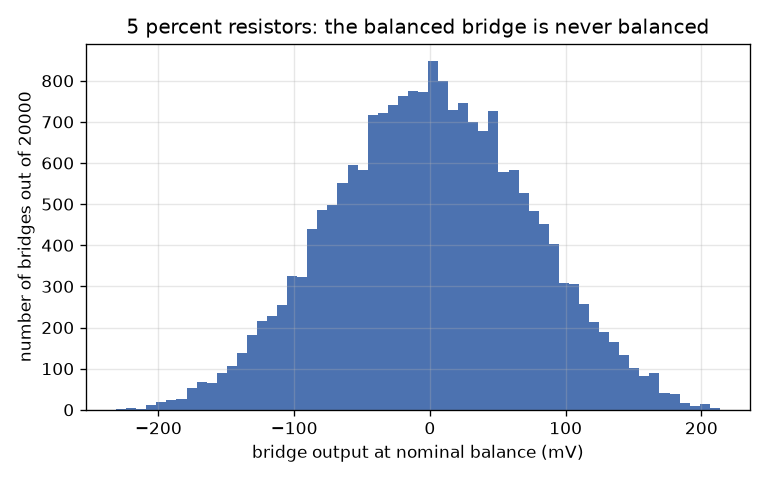
\includegraphics[width=0.85\linewidth]{figures/s03_bridge_tolerance.png}\\\small Output of 20000 nominally balanced bridges with 5 percent resistors on 5 V.\end{center}

\subsection*{E. Worked example}
A 12 V source feeds R1 = 1 kohm in series with R2 = 2 kohm to ground. Find the Thevenin equivalent seen across R2, then the current, voltage and power in a 1 kohm load, and compare with the maximum power the network can ever deliver. Verify with one nodal equation.
\begin{enumerate}[nosep]
\item V\_th = open-circuit voltage across R2 = 12 * 2 / (1 + 2) = 8 V.
\item R\_th: switch the source off (replace by a wire); R1 and R2 are then in parallel: 1000 * 2000 / 3000 = 666.7 ohm.
\item With a 1 kohm load: I = 8 / (666.7 + 1000) = 4.8 mA, V\_load = 4.8 mA * 1 kohm = 4.8 V, P = 4.8 * 4.8 mA = 23.04 mW.
\item Maximum power: P\_max = 8\textasciicircum{}2 / (4 * 666.7) = 24.0 mW, at R\_L = 666.7 ohm. The 1 kohm load gets 96 percent of that.
\item Nodal check with the node between the resistors: (v - 12)/1000 + v/2000 + v/1000 = 0, so v * 0.0025 = 0.012 and v = 4.8 V. It agrees with V\_load.
\end{enumerate}
\textbf{Answer.} V\_th = 8 V, R\_th = 666.7 ohm; the 1 kohm load gets 4.8 V, 4.8 mA and 23.04 mW; the maximum possible is 24.0 mW at R\_L = 666.7 ohm.

\subsection*{F. Questions}
\begin{enumerate}[nosep]
\item \textbf{Conceptual.} Why does a circuit with a node that is not connected to the reference node (a floating node) make G singular, and what does the error mean physically?
\item \textbf{Numerical.} For the 12 V, 1 kohm and 2 kohm network of Section E find the load that would receive 20 mW. Is there more than one answer? Check against P\_max.
\item \textbf{Graph and simulation interpretation.} In the histogram of 20000 bridges with 5 percent resistors on 5 V, the standard deviation is 72 mV. A 1 percent change of one arm gives a signal of 12.4 mV. What does this tell you about using 5 percent resistors for a sensor, and what would change with 1 percent resistors?
\item \textbf{Design and optimisation challenge.} Design: the Pt1000 bridge needs at least 100 mV at 100 degrees C and at most 1 mW in the sensor, with three fixed 1 kohm resistors. Choose the supply voltage, justify it, and say what limits the accuracy at 5 percent tolerance.
\end{enumerate}

\section{Real-world mini-project}
\textbf{Design a Pt1000 temperature-sensor bridge.} A Pt1000 sensor has the resistance 1000 (1 + 0.00385 T) ohm for a temperature T in degrees Celsius (a straight-line approximation). Put it in one arm of a Wheatstone bridge whose other three resistors are 1000 ohm, so the bridge is balanced at 0 degrees C. You choose only the supply voltage in steps of 0.1 V between 1.0 V and 5.0 V. Requirements: the output at 100 degrees C must be at least 100 mV, and the heat in the sensor at 100 degrees C must not exceed 1 mW (more heat warms the sensor and falsifies the reading). Use \texttt{sensor\_bridge\_out}, \texttt{sensor\_power} and \texttt{monte\_carlo\_bridge} from Session 3.

\section{The path ahead}
\begin{enumerate}[nosep]
\item \textbf{Session 4: Read a netlist.} A function that reads lines such as 'R1 1 2 1k' and 'V1 1 0 12' and returns the input of the solver.
\item \textbf{Session 5: A nonlinear part: the diode.} A diode stamp linearised at each iteration, solved inside a loop around the nodal solver.
\item \textbf{Session 6: An amplifier from a controlled source.} A controlled-source stamp and an inverting amplifier built with it.
\item \textbf{Session 7: Sensitivity without Monte Carlo.} A function returning dVout/dR for every resistor of any network.
\item \textbf{Session 8: Time enters: the RC circuit.} A transient solver for a resistor and a capacitor on a step input.
\end{enumerate}

\section{Answers and hints}

\subsection*{Session 1}
\begin{enumerate}[nosep]
\item \textbf{Conceptual.} Hint: A current needs a closed loop. How many loops are there in each wiring? Solution: In a series string there is only one path for the current. A broken filament is a gap in that path, so the current is zero everywhere and every bulb goes dark. In a parallel string each bulb has its own path straight across the battery. A gap in one path does not affect the others, so they keep their full voltage and stay lit (the battery just supplies a little less current).
\item \textbf{Numerical.} Hint: Series: R\_total = N R. Parallel: each bulb has the full 9 V. Then P = V I. Solution: Series: R\_total = 30 ohm, I = 9 / 30 = 0.3 A, each bulb gets 3 V and P = 3 * 0.3 = 0.9 W. Parallel: each bulb gets 9 V, I per bulb = 0.9 A, P = 9 * 0.9 = 8.1 W, battery current 2.7 A. Sanity check: parallel is 9 times brighter than series for 3 bulbs (N\textasciicircum{}2 = 9), and 0.9 * 9 = 8.1.
\item \textbf{Graph and simulation interpretation.} Hint: Find the blue and green curves at N = 4. Solution: At N = 4 the green (parallel) curve is at 3.6 W and the blue (series) curve at 0.225 W. The ratio is 3.6 / 0.225 = 16 = N\textasciicircum{}2. The blue curve falls like 1 / N\textasciicircum{}2, the green one is flat.
\item \textbf{Design and optimisation challenge.} Hint: Compute the battery current and the power in each bulb for each wiring. Solution: All series: I = 0.2 A, 0.4 W per bulb: allowed. All parallel: I = 1.8 A, which is above the 1 A limit: not allowed. One bulb in series with a pair in parallel: R = 10 + 5 = 15 ohm, I = 0.4 A; the lone bulb gets 4 V and 1.6 W, each bulb of the pair 2 V and 0.4 W: allowed, and brighter overall, but unevenly. All series is the simplest and gives equal brightness; the mixed wiring gives more light at the cost of unequal bulbs and a failure of the lone bulb putting the whole circuit out. Assumption: ideal battery and fixed bulb resistance.
\end{enumerate}

\subsection*{Session 2}
\begin{enumerate}[nosep]
\item \textbf{Conceptual.} Hint: What happens to the resistance of the lower part when a load is put across it? Solution: The load is in parallel with R2, and a parallel combination is always smaller than either part: R2 \textbar{}\textbar{} R\_L \textless{} R2. A smaller lower resistance takes a smaller share of the input voltage, so V\_out falls. The load can be ignored when R\_L is much larger than R2 (a common rule is at least 10 times larger): then R2 \textbar{}\textbar{} R\_L is only slightly smaller than R2.
\item \textbf{Numerical.} Hint: With the load, the lower resistance is 1 kohm \textbar{}\textbar{} 1 kohm. Solution: Unloaded: 9 * 1 / (2 + 1) = 3.0 V. With the load: the lower part is 0.5 kohm, so V\_out = 9 * 0.5 / (2 + 0.5) = 1.8 V. KVL check: the current is 9 / 2.5 kohm = 3.6 mA, drop across R1 = 3.6 mA * 2 kohm = 7.2 V, and 7.2 + 1.8 = 9 V. The load took 40 percent of the output voltage away.
\item \textbf{Graph and simulation interpretation.} Hint: The curve crosses 3.0 V between the readings at 10 kohm (2.967 V) and 47 kohm (3.223 V). Solution: The output is 3.0 V when the lower part is 2550 ohm, which needs R\_L = 2550 * 3300 / (3300 - 2550) = 11.2 kohm: the curve crosses 3.0 V between 10 and 47 kohm, at about 11 kohm. Making R2 smaller lowers the whole curve (the unloaded value falls) but flattens it, since a smaller R2 is less disturbed by the same load. Reading the units: the x axis is ohm, the y axis volts.
\item \textbf{Design and optimisation challenge.} Hint: Use R\_low = R1 * 3.3 / 1.7 and then 1 / R2 = 1 / R\_low - 1 / R\_L, or call design\_r2 and stiffness\_table in lesson.py. Solution: R1 = 220: R2 = 469.7 ohm, source current 7.73 mA, unplugging the load raises the output by 0.105 V. R1 = 470: R2 = 1132 ohm, 3.62 mA, +0.233 V. R1 = 1000: R2 = 3307 ohm, 1.70 mA, +0.539 V. Small resistors give a stiff divider (little change with the load) but waste current and heat; large resistors save current but change a lot if the load changes. A reasonable compromise is R1 = 470 or 1000 ohm depending on the battery budget; with a fixed load, R1 = 1000 and the standard 3.3 kohm (output 3.299 V, 1.7 mA) is within 0.1 percent. R1 = 4700 is impossible: the load alone would pull the output below the target.
\end{enumerate}

\subsection*{Session 3}
\begin{enumerate}[nosep]
\item \textbf{Conceptual.} Hint: What fixes the voltage of a node? What happens to all voltages if you add 1 V to every node of the floating part? Solution: Only voltage differences matter to resistors. If a group of nodes has no path to the 0 V reference, adding the same voltage to all of them changes no current, so the equations cannot fix their absolute voltage: G has a zero eigenvalue, it is singular, and there are infinitely many solutions. Physically the floating part has no defined voltage: connect it to the reference (or add a reference resistor) to make it solvable. Two different ideal sources across the same two nodes are also singular: they demand two voltages at once.
\item \textbf{Numerical.} Hint: Solve V\_th\textasciicircum{}2 R\_L / (R\_th + R\_L)\textasciicircum{}2 = 0.020 with V\_th = 8 V and R\_th = 666.7 ohm; it is a quadratic in R\_L. Solution: 64 R\_L = 0.020 (R\_th + R\_L)\textasciicircum{}2 gives R\_L\textasciicircum{}2 + (2 R\_th - 3200) R\_L + R\_th\textasciicircum{}2 = 0, that is R\_L\textasciicircum{}2 - 1866.7 R\_L + 444444 = 0. The roots are R\_L = (1866.7 +- sqrt(1866.7\textasciicircum{}2 - 4 * 444444)) / 2 = (1866.7 +- 1306.4)/2 = 280.2 ohm and 1586.5 ohm. Two answers, one on each side of R\_th = 666.7, since 20 mW is less than P\_max = 24 mW. A target above 24 mW would have no solution.
\item \textbf{Graph and simulation interpretation.} Hint: Compare the spread with the signal. The spread scales with the tolerance. Solution: The offset error (72 mV, one standard deviation) is about six times larger than the signal from a 1 percent change in the sensor: the unadjusted bridge cannot resolve small changes, and only about 11 percent of bridges are within 10 mV of zero. With 1 percent resistors the spread shrinks 5 times to about 14 mV. In practice the zero offset is measured once and subtracted (calibration), or one arm is trimmed with a potentiometer.
\item \textbf{Design and optimisation challenge.} Hint: Use sensor\_bridge\_out(vs, 100) and sensor\_power(vs, 100) for supply voltages in steps of 0.1 V, then run monte\_carlo\_bridge. Solution: The output is 80.7 mV per volt of supply, so 100 mV needs at least 1.3 V; the sensor heat grows as Vs squared (0.244 mW per V squared), so 1 mW allows at most 2.0 V. Any supply from 1.3 V to 2.0 V works; 2.0 V gives the largest signal (161 mV at 100 degrees C, 0.97 mW), while 1.5 V gives 121 mV and 0.55 mW with a safer margin on self-heating. The limit is the tolerance: at 2.0 V the 5 percent resistors give a zero offset of 29 mV (about 15 degrees C of equivalent error), 1 percent parts about 5.8 mV (about 3 degrees C). Trade-off: higher supply, more signal, more self-heating; tighter parts cost more. Assumption: linear Pt1000 model and no amplifier noise.
\end{enumerate}

\section{How to join}
Read \texttt{CONTRIBUTING.md} in the repository, then pick an issue labelled \texttt{good first issue}. Repository: \url{https://github.com/KrunalPanchal1995/opencircuitlab}

\end{document}
